\chapter{Experiments}
In this chapter describe the two main experiments we built to collect data and analyze our system. Ten people were involved in the data collection. Each experiment will be presented in terms of goals, procedures and results (either qualitative or quantitative).
\section{Pointing Feedback}
\subsection{Setup}
\begin{figure}
	\centering
	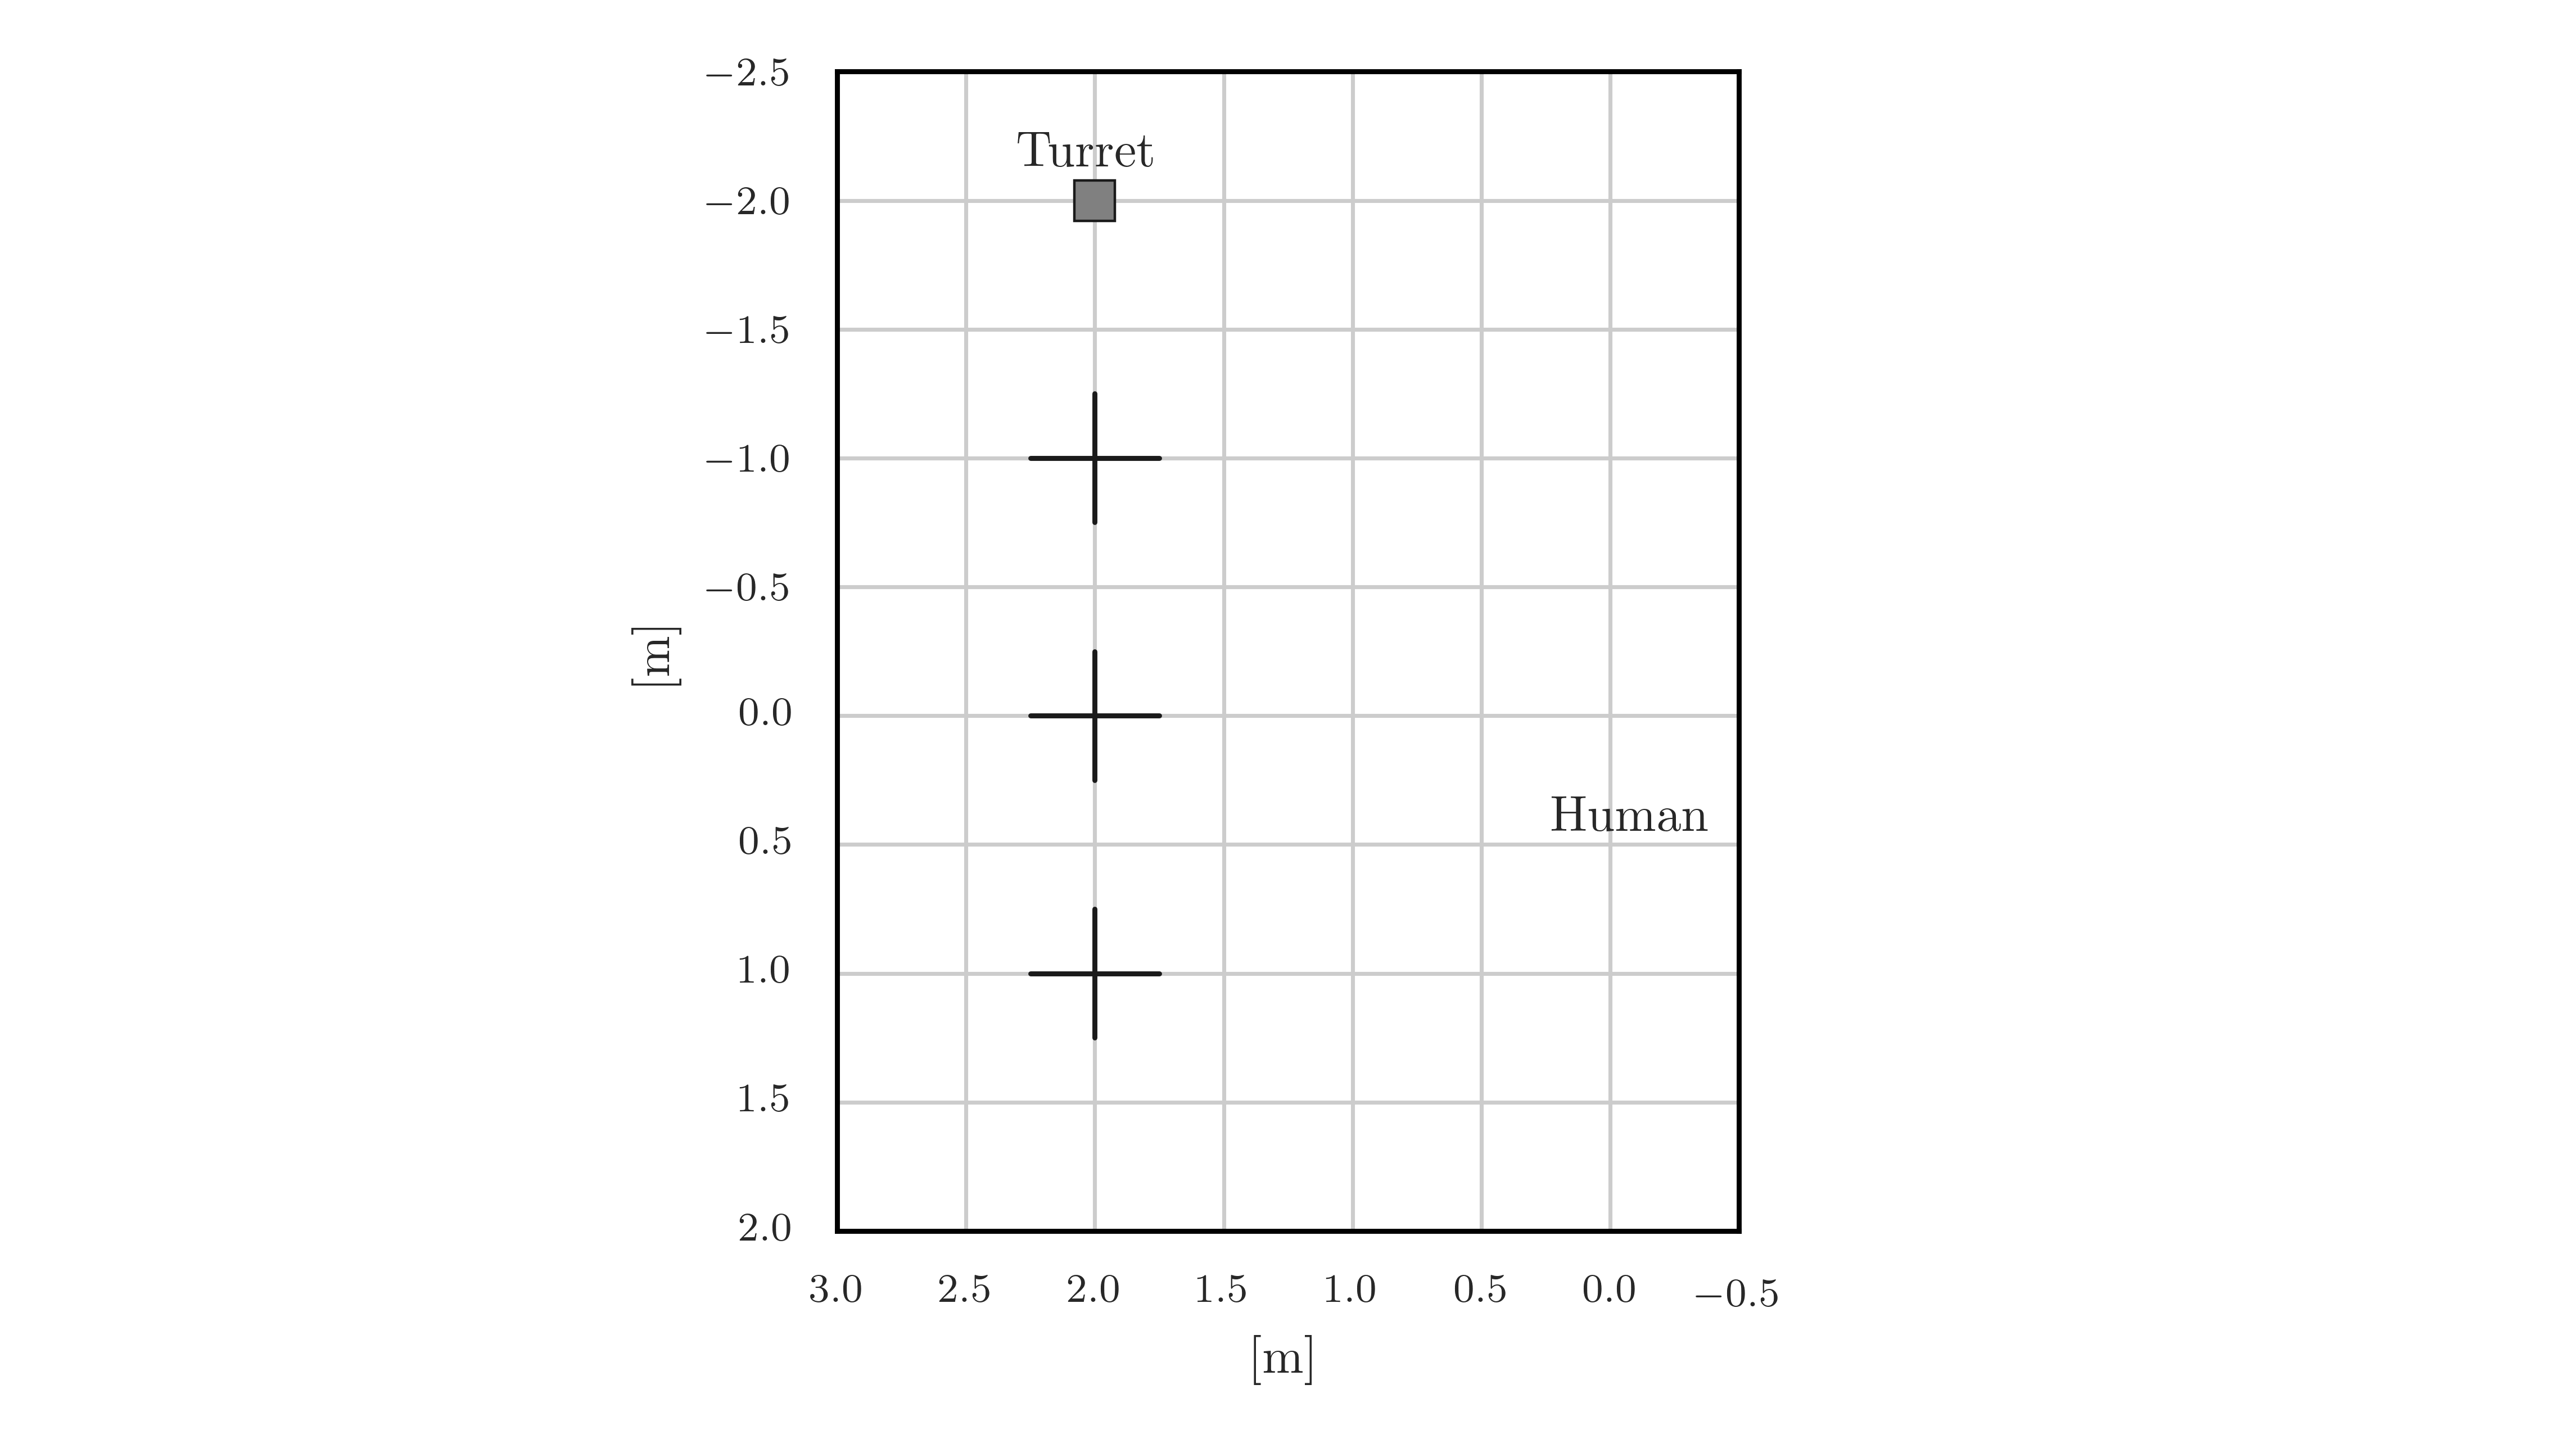
\includegraphics[width=\textwidth]{img/pointingExpSetup.png}%
	\caption{Pointing Experiment Setup}
	\label{fig:pointingExpSetup}
\end{figure}
We place the turret and three ground targets in known positions. The user is placed in front of the second target, oriented perpendicularly to the line connecting the targets. Figure \ref{fig:pointingExpSetup} shows that setup. The relative localization between the human and the turret is known a priori, so we are not performing any relloc. The user is wearing the IMU and we are collecting his pointing data.\\
The user has to point each target first without any additional visual feedback, so he has to rely solely on his perception. Second, he has to point again with the visual feedback provided by the laser dot. Those are the steps composing each iteration of the experiment (one for each target):
\begin{itemize}
    \item after a countdown, the user points the target without feedback;
    \item the user keeps pointing for 5 seconds
    \item after a sound feedback, the user can rest his arm;
    \item after a countdown, the user points the target with the laser feedback;
    \item the user keeps pointing for 5 seconds
    \item after a sound feedback, the user can rest his arm.
\end{itemize}
Each user has to perform that loop three time for each target, for a total of nine iterations.
\subsection{Goals}
The performance of the interface crucially relies on operator’s perception. Due to simplifications in the pointing model that we use and various sensory errors, the estimated frame transformations and the pointing are expected to be imprecise.\\
With that experiment we want to understand if availability of visual feedback is useful and thus improves the pointing accuracy. This is why we ask users to drive the laser dot to the target, where the laser dot represents the location where the system thinks the user is pointing. Comparing results with and without feedback, we can understand if providing that feedback helps users to timely adapt to any misalignments.

\subsection{Quantitative Results}
First, we can look at the users' trajectories with and without feedback in figure \ref{fig:userTrajectories}. We can immediately see that without feedback users go straight to their goal point, but that point, for the system, does not correspond to the target. With feedback, on the contrary, users are able to tell the system to point at the target. This intuition is confirmed by figure \ref{fig:avgDistance}: without feedback, users quickly reach an average distance from the target of 0.5 m but do not improve any further. When the feedback is provided, distance decreases to almost 0 within 5 seconds. This is expected as the system has intrinsic inaccuracies (for example in the reconstruction of pointing rays) which the user is unable to see and correct. 

This demonstrates that real-time feedback is a key component for our system. This justifies all the work done to build the turret, as, while with fast moving robots (e.g. a drone), the robot position itself can be the feedback, for slow moving machine (e.g. a ground robot) the laser dot represents a valid possibility, as also our demos with the kobuki show.

\begin{figure}
	\centering
	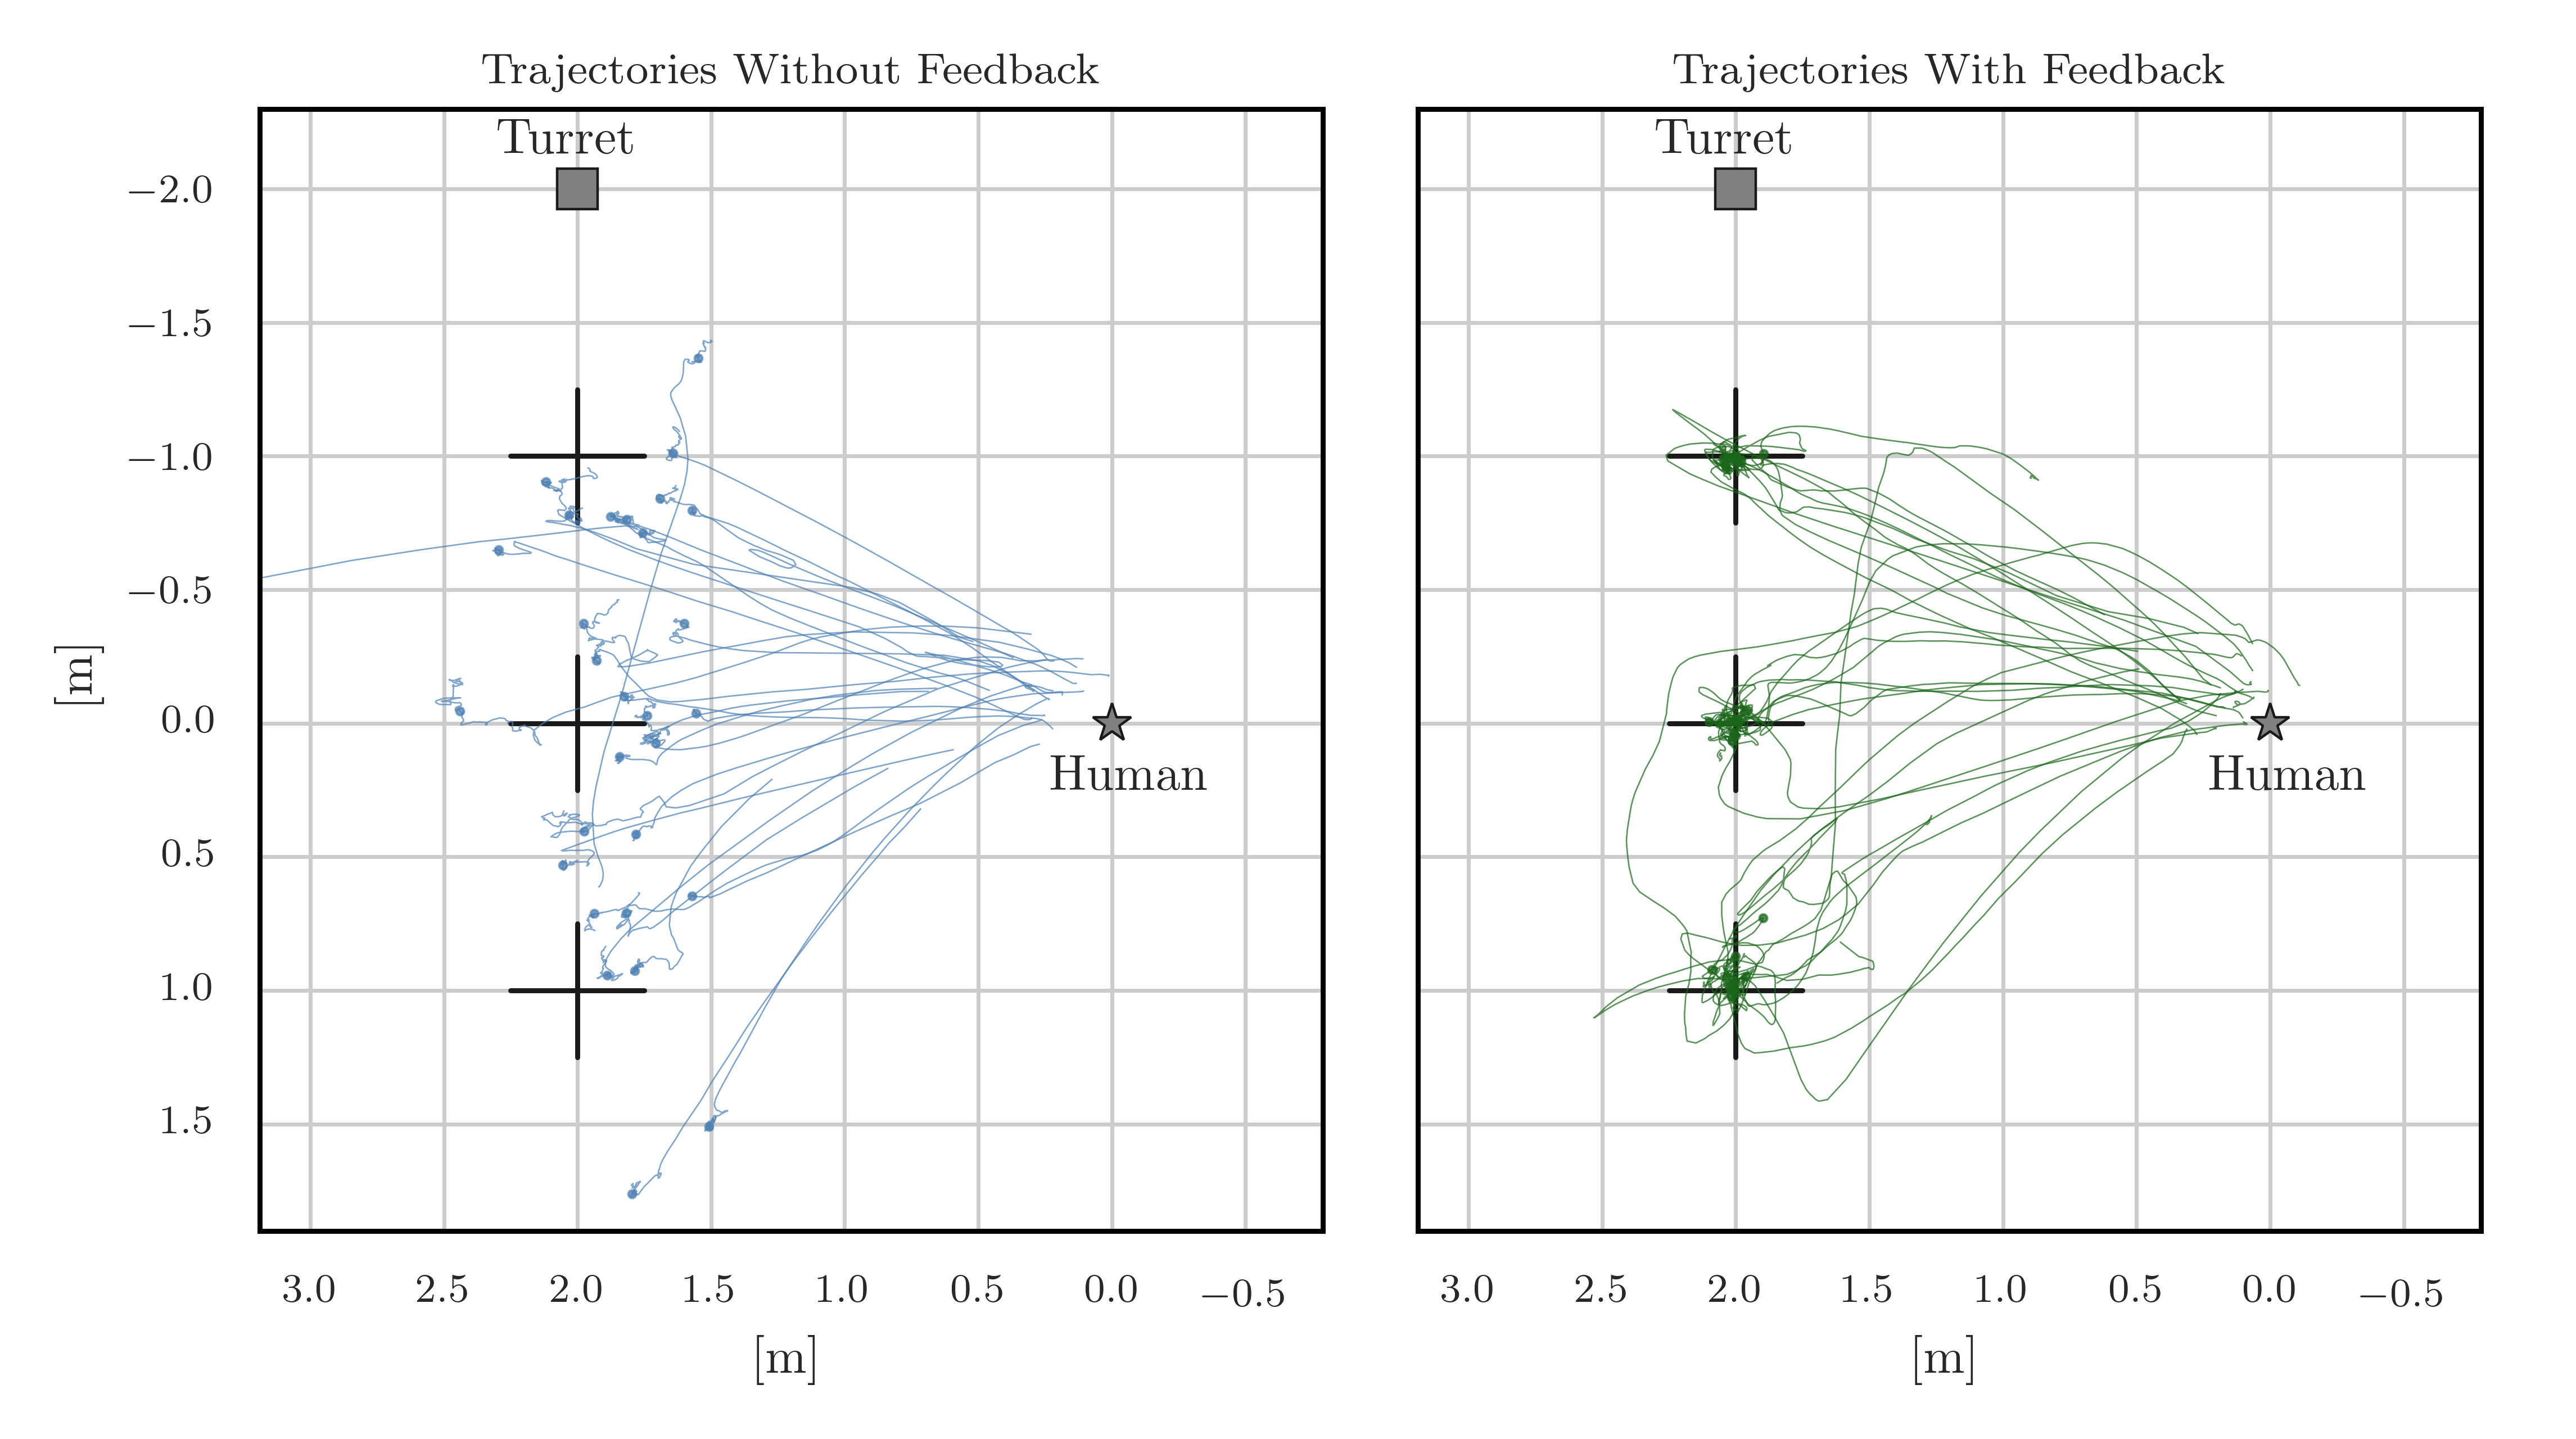
\includegraphics[width=\textwidth]{img/userTrajectories.png}%
	\caption{Users' Trajectories With and Without Feedback}
	\label{fig:userTrajectories}
\end{figure}
\begin{figure}
	\centering
	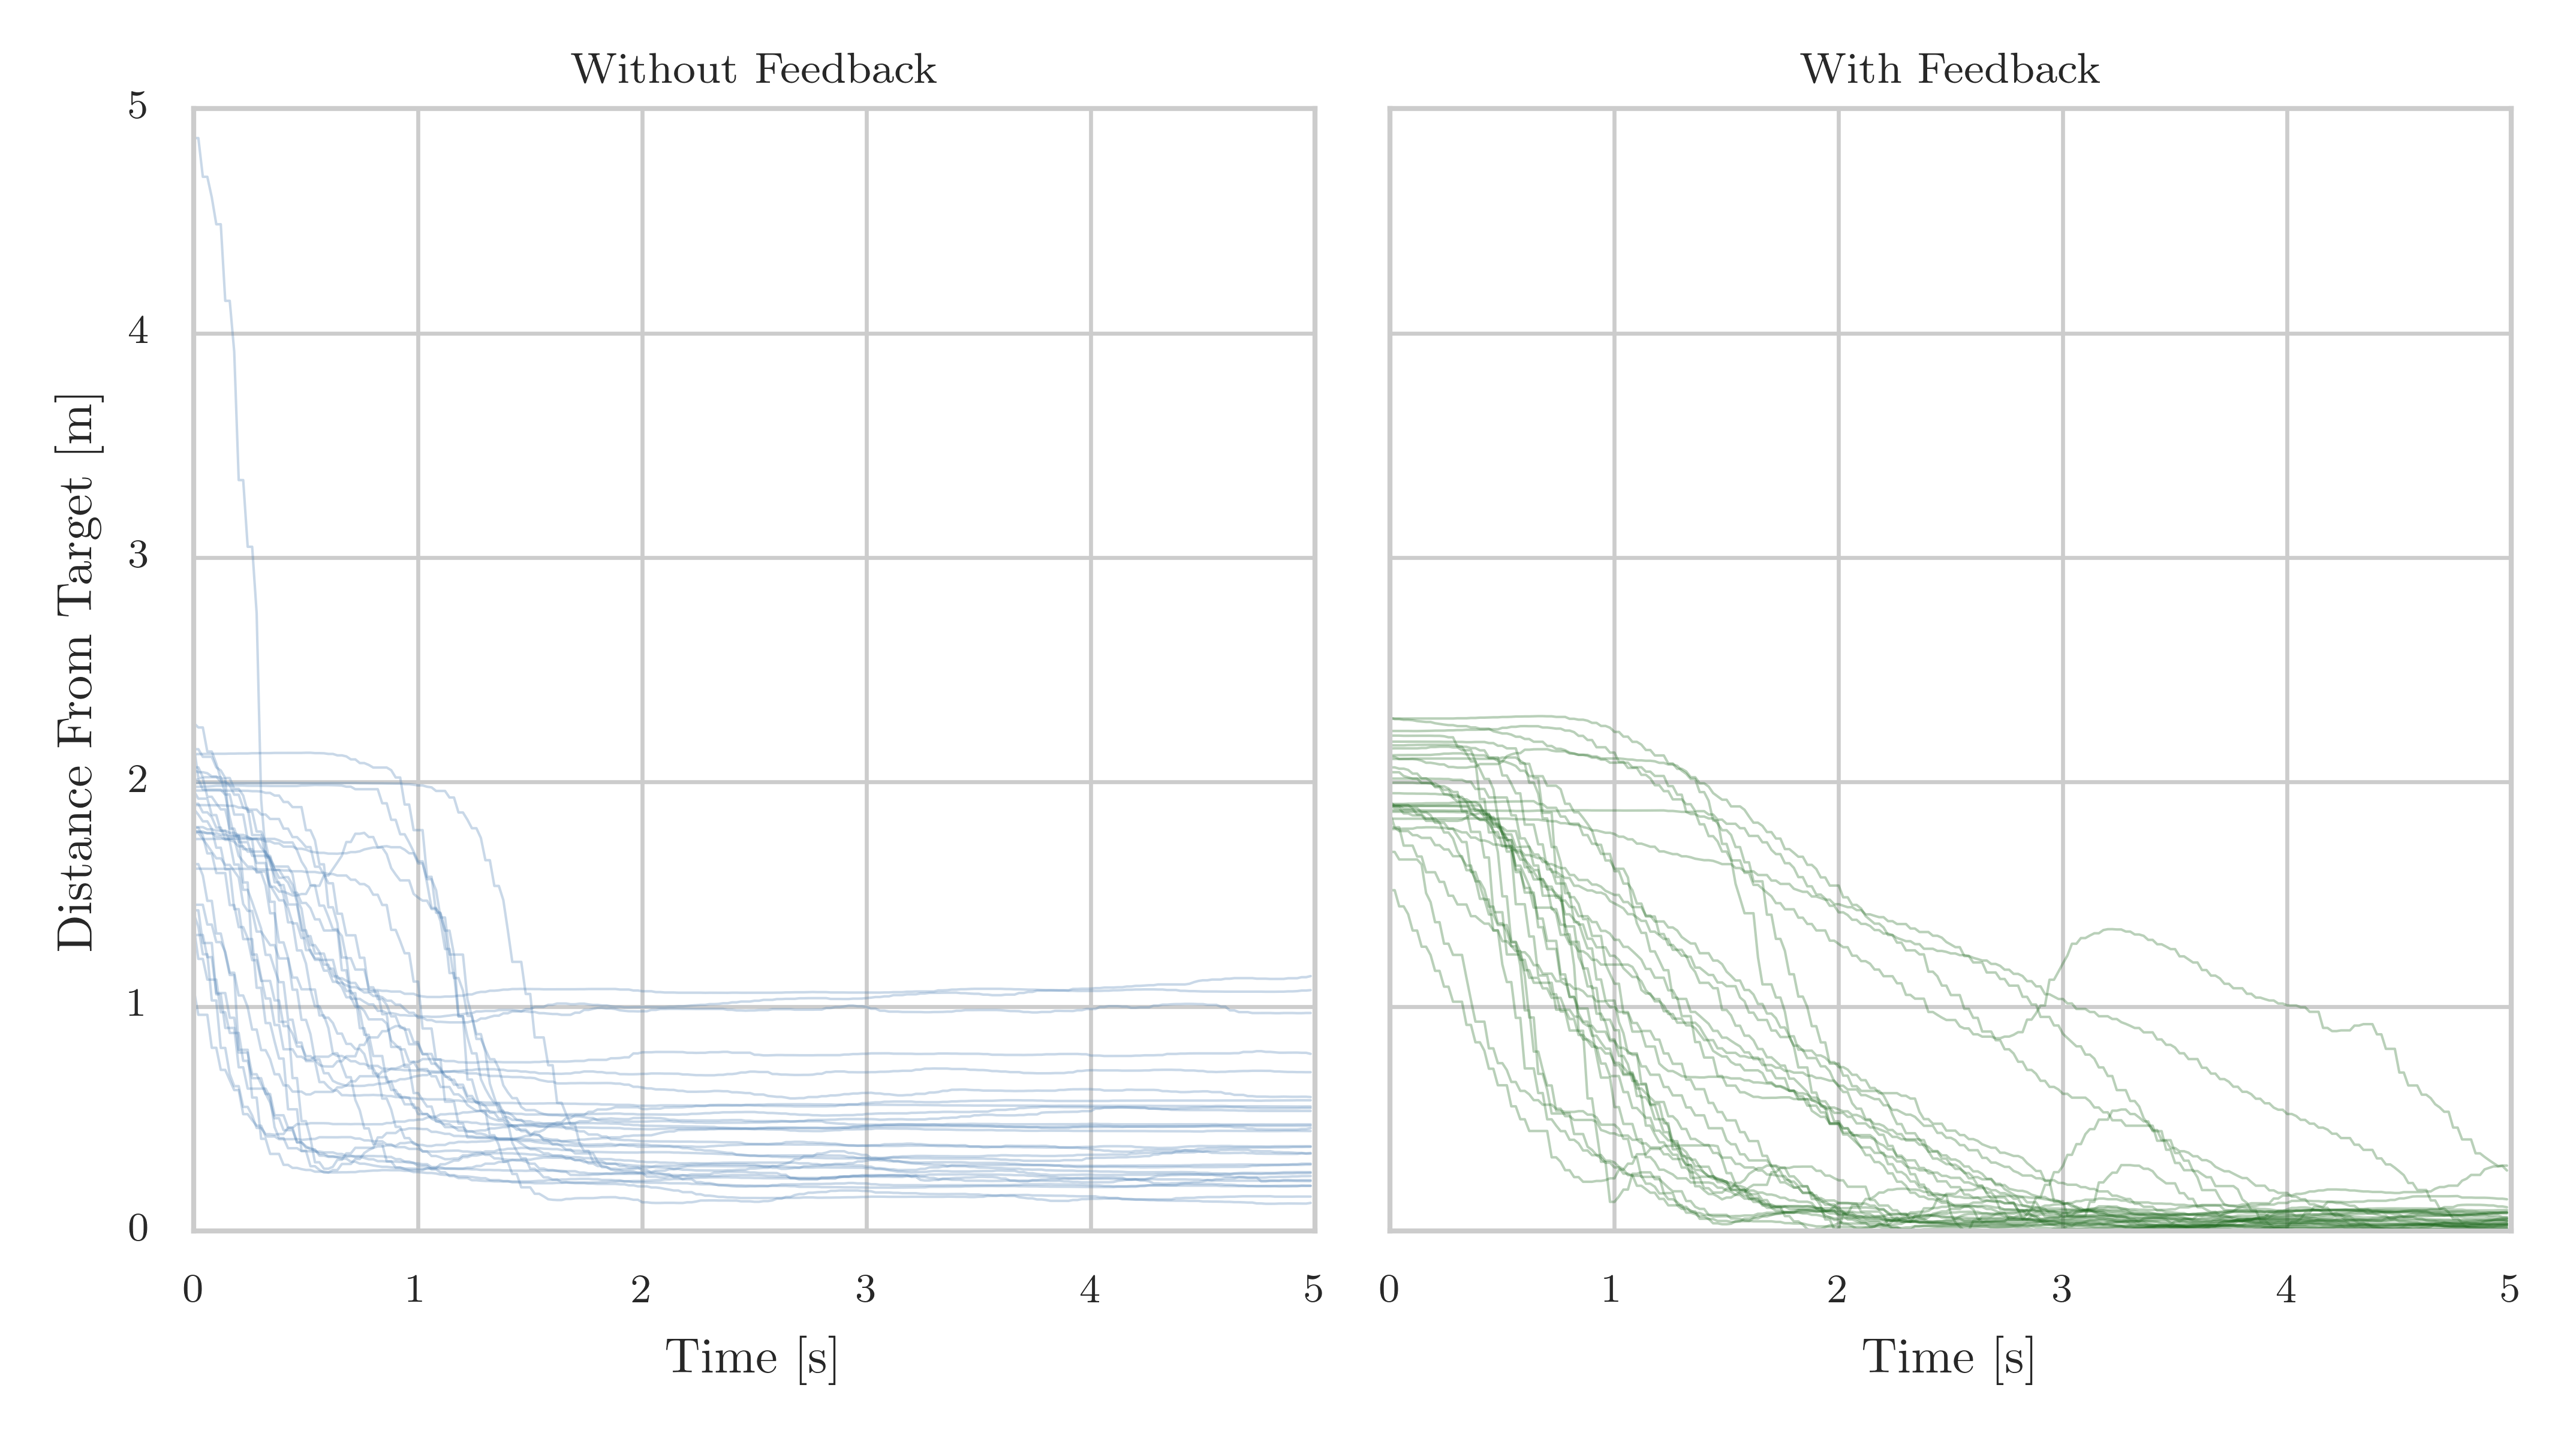
\includegraphics[width=\textwidth]{img/distanceComparison.png}%
	\caption{Comparison Of Distances Over Time}
	\label{fig:distanceComparison}
\end{figure}
\begin{figure}
	\centering
	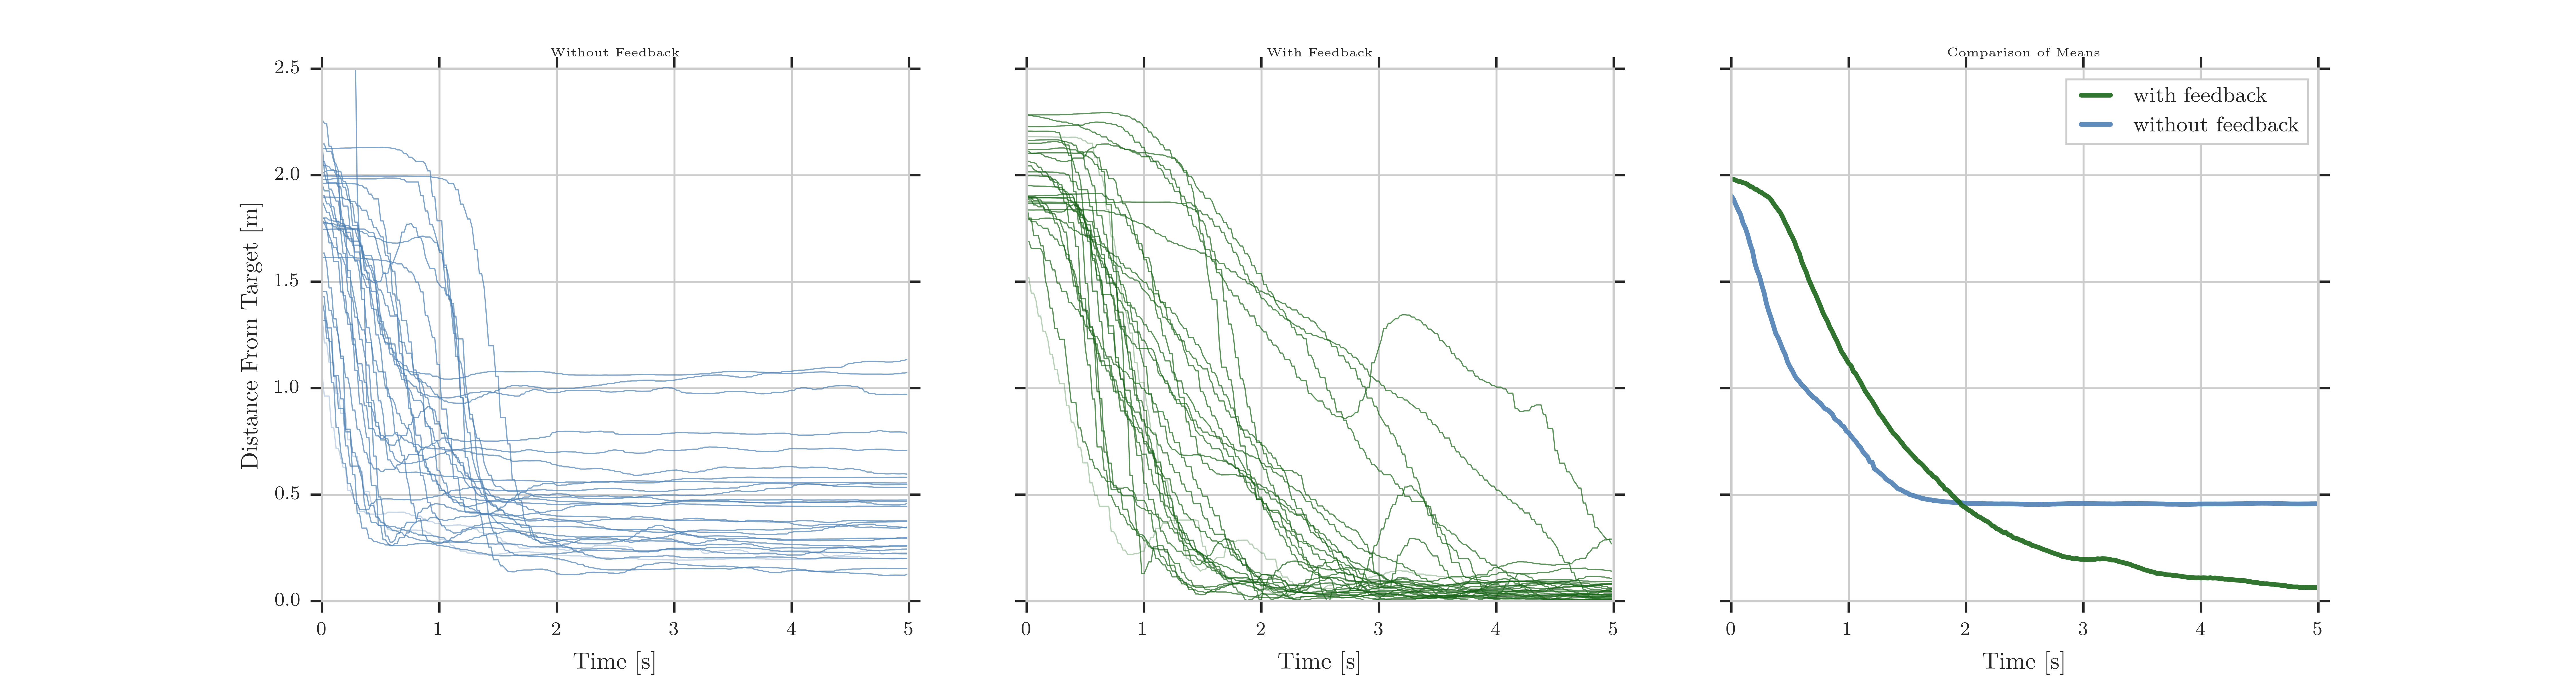
\includegraphics[width=\textwidth]{img/avgDistance.png}%
	\caption{Comparison Of Average Distances Over Time}
	\label{fig:avgDistance}
\end{figure}